\section{LQG control}
\subsection{Introduction LQG}
In the previous sections it was assumed that the state vectors where know. In reality this is rarely the case as the controller is controlling a physical device. Which can be approximated with a model but only the inputs and outputs can be directly measured. The internal states can be estimated trough system identification, which is exactly what the Kalman filter does. It estimates the internal states based on the current and past inputs and outputs.

The diagram Figure~\ref{fig:diagram LQG controller} illustrates how the Kalman filter is integrated in the circuit. The quad copter states x(t) are not used in implementing the controller this time, only the outputs and inputs are used. 
\begin{figure}[H]
	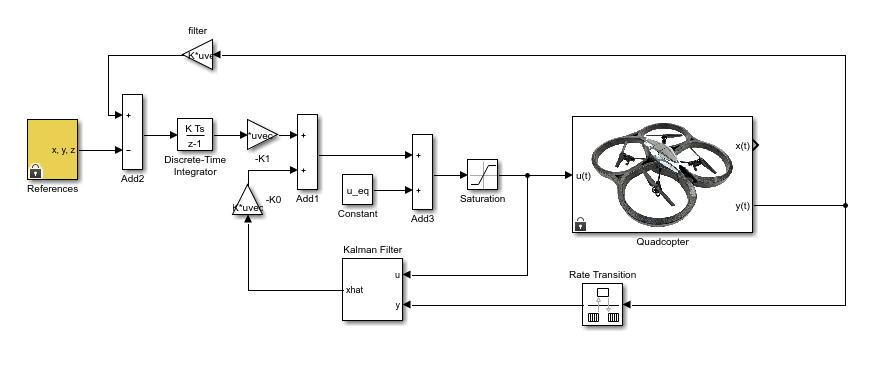
\includegraphics[width=\textwidth]{./LQG/diagram_LQG.png}
	\caption{LQG controller}
	\label{fig:diagram LQG controller}
\end{figure}
\subsection{Designing the Kalman filter}
The Kalman filter uses the same linear model as the controller does but it must take in account the noise on the state and output. The assignment states that system should be interpreted as equation~\ref{eq:basic system with noise} .The only parameter that needs to be calculated is the L from equation~\ref{eq:basic equation kalman}.

\begin{equation}
	x_{k+1} = Ax_k + Bu_k +w_k \\
	y_k = Cx_k + Du_k + v_k
	\label{eq:basic system with noise}
\end{equation}

\begin{equation}
x_{k+1|k} = A\hat{x}_{k|k-1} + Bu_k + L(y_k - C\hat{x}_{k|k-1} - Du_k)
\label{eq:basic equation kalman}
\end{equation}

\begin{eqnarray}
	E(w_jw_k^T) = Q \delta_{jk} \\
	E(v_jv_k^T) = R \delta_{jk}
\end{eqnarray}

If the noise w and v is assumed to be white Gaussian noise with the given variance from the assignment the matrix

output noise:
$$
R=\begin{bmatrix}
2.5 \cdot 10^{-5} & 0 & 0 & 0 & 0 & 0 \\
0 & 2.5 \cdot 10^{-5} & 0 & 0 & 0 & 0 \\
0 & 0 & 2.5 \cdot 10^{-5} & 0 & 0 & 0 \\
0 & 0 & 0 & 7.57 \cdot 10^{-5} & 0 & 0 \\
0 & 0 & 0 & 0 & 7.57 \cdot 10^{-5} & 0 \\
0 & 0 & 0 & 0 & 0 & 7.57 \cdot 10^{-5} \\
\end{bmatrix}
$$
state noise:
$$
Q=\begin{bmatrix}
10^{-1} & 0 & 0 & 0 & 0 & 0 & 0 & 0 & 0 & 0 & 0 & 0 & 0 & 0 & 0 \\
0 & 10^{-1} & 0 & 0 & 0 & 0 & 0 & 0 & 0 & 0 & 0 & 0 & 0 & 0 & 0 \\
0 & 0 & 10^{-1} & 0 & 0 & 0 & 0 & 0 & 0 & 0 & 0 & 0 & 0 & 0 & 0 \\
0 & 0 & 0 & 10^{-3} & 0 & 0 & 0 & 0 & 0 & 0 & 0 & 0 & 0 & 0 & 0 \\
0 & 0 & 0 & 0 & 10^{-3} & 0 & 0 & 0 & 0 & 0 & 0 & 0 & 0 & 0 & 0 \\
0 & 0 & 0 & 0 & 0 & 10^2 & 0 & 0 & 0 & 0 & 0 & 0 & 0 & 0 & 0 \\
0 & 0 & 0 & 0 & 0 & 0 & 10^{-3} & 0 & 0 & 0 & 0 & 0 & 0 & 0 & 0 \\
0 & 0 & 0 & 0 & 0 & 0 & 0 & 10^{-3} & 0 & 0 & 0 & 0 & 0 & 0 & 0 \\
0 & 0 & 0 & 0 & 0 & 0 & 0 & 0 & 10^{-3} & 0 & 0 & 0 & 0 & 0 & 0 \\
0 & 0 & 0 & 0 & 0 & 0 & 0 & 0 & 0 & 10^{-3} & 0 & 0 & 0 & 0 & 0 \\
0 & 0 & 0 & 0 & 0 & 0 & 0 & 0 & 0 & 0 & 10^{-3} & 0 & 0 & 0 & 0 \\
0 & 0 & 0 & 0 & 0 & 0 & 0 & 0 & 0 & 0 & 0 & 10^{-3} & 0 & 0 & 0 \\
0 & 0 & 0 & 0 & 0 & 0 & 0 & 0 & 0 & 0 & 0 & 0 & 10^{-3} & 0 & 0 \\
0 & 0 & 0 & 0 & 0 & 0 & 0 & 0 & 0 & 0 & 0 & 0 & 0 & 10^{-3} & 0 \\
0 & 0 & 0 & 0 & 0 & 0 & 0 & 0 & 0 & 0 & 0 & 0 & 0 & 0 & 10^{-3} \\
\end{bmatrix}
$$

\subsection{Simulation without weight}
The same weight matrices from the integrator will be used.

The output noise is in the range of $10^{-5}$ this seems like a good place to start. So an diagonal matrix with $10^{-5}$ is taken as starting point. After a few tries it becomes clear that $10^-{3}$ seems to give the best results displayed in figure~\ref{fig:LQG step 1}.

\begin{figure}[H]
	\centering
	\begin{subfigure}[b]{0.3\textwidth}
		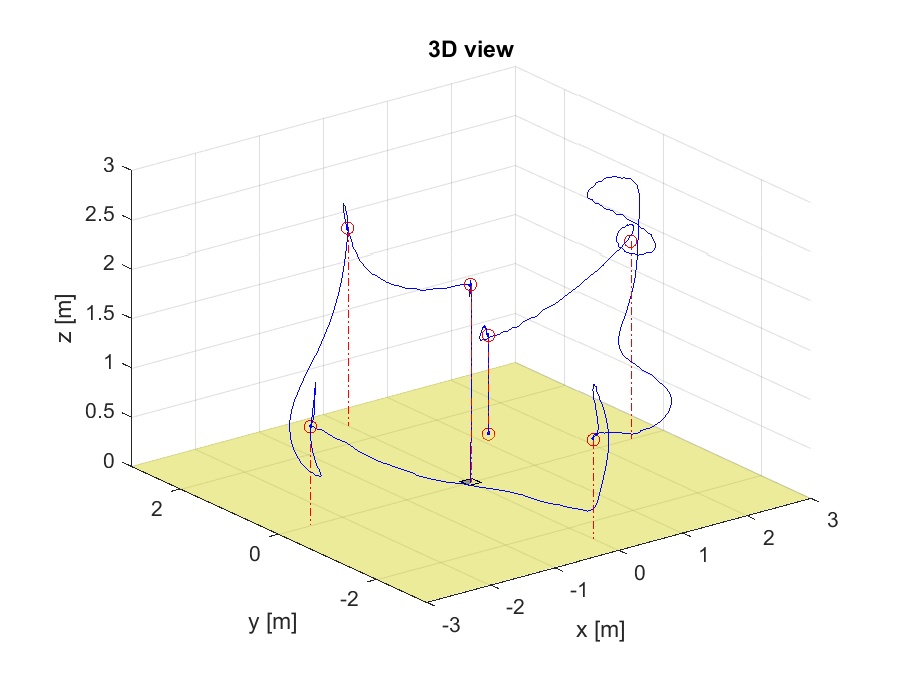
\includegraphics[width=\textwidth]{./LQG/kalman_covar/fig2_init.eps}
		\caption{3D view}
	\end{subfigure}
	\begin{subfigure}[b]{0.3\textwidth}
		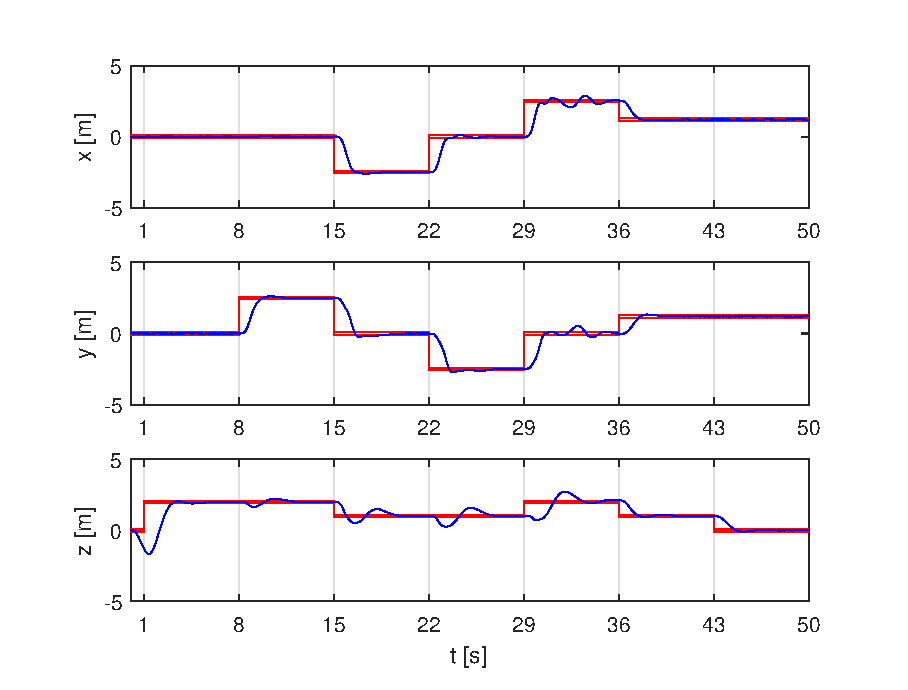
\includegraphics[width=\textwidth]{./LQG/kalman_covar/fig3_init.eps}
		\caption{individual axis}
	\end{subfigure}
	\caption{LQG controller with Q taken as a diagonal matrix with $10^-3$ on its diagonal}\label{fig:LQG step 1}
\end{figure}

The oscillations on the x,y and z axis on figure~\ref{fig:LQG step 1} are partially due to the integrator. It over steers the motors this is the same problem as with determining the matrices for the integrator LQR controller. The first 3 diagonal elements of the Q matrix are increased from $10^{-3}$ to $10^{-1}$. An other way of looking at it is that the integrator adds the difference on x,y and z, and the numerical error on adding numbers is the sum of the absolute errors.

This however is not sufficient to fix the z-axis increasing the variance even further does not improve the results by a lot. Maybe the variance on the  state of z-axis is actually larger. By increasing the 6th diagonal element from $10^-3$ to $10^2$ there is an significant improvement on the z-axis. The voltages send to the motors however is staring to oscillate so going higher then $10^2$ will increase the results but robustness will be lost. The final results are displayed in figure~\ref{fig:LQG without weight final}.

The surprising thing about the final result is that the average time is about the same as with using the actual states instead of the kalman filter. However the system output is a bit more nervous. 

\begin{figure}[H]
	\centering
	\begin{subfigure}[b]{0.3\textwidth}
		\includegraphics[width=\textwidth]{./LQG/kalman_covar/fig1.eps}
		\caption{top view}
	\end{subfigure}
	\begin{subfigure}[b]{0.3\textwidth}
		\includegraphics[width=\textwidth]{./LQG/kalman_covar/fig2.eps}
		\caption{3D view}
	\end{subfigure}
	\begin{subfigure}[b]{0.3\textwidth}
		\includegraphics[width=\textwidth]{./LQG/kalman_covar/fig3.eps}
		\caption{individual axis}
	\end{subfigure}
	\begin{subfigure}[b]{0.3\textwidth}
		\includegraphics[width=\textwidth]{./LQG/kalman_covar/fig4.eps}
		\caption{angles}
	\end{subfigure}
	\begin{subfigure}[b]{0.3\textwidth}
		\includegraphics[width=\textwidth]{./LQG/kalman_covar/fig5.eps}
		\caption{actions}
	\end{subfigure}
	\caption{LQG with the final Q and R, average time 2.893s}\label{fig:LQG without weight final}
\end{figure}


\subsection{simulation with weight}
The result of the quad copter with 0.1 weight is displayed in figure~\ref{fig:LQG with weight}. The average run time is again about the same as with the actual states instead of the kalman filter. 
\begin{figure}[H]
	\centering
	\begin{subfigure}[b]{0.3\textwidth}
		\includegraphics[width=\textwidth]{./LQG/with_weight/fig1.eps}
		\caption{top view}
	\end{subfigure}
	\begin{subfigure}[b]{0.3\textwidth}
		\includegraphics[width=\textwidth]{./LQG/with_weight/fig2.eps}
		\caption{3D view}
	\end{subfigure}
	\begin{subfigure}[b]{0.3\textwidth}
		\includegraphics[width=\textwidth]{./LQG/with_weight/fig3.eps}
		\caption{individual axis}
	\end{subfigure}
	\begin{subfigure}[b]{0.3\textwidth}
		\includegraphics[width=\textwidth]{./LQG/with_weight/fig4.eps}
		\caption{angles}
	\end{subfigure}
	\begin{subfigure}[b]{0.3\textwidth}
		\includegraphics[width=\textwidth]{./LQG/with_weight/fig5.eps}
		\caption{actions}
	\end{subfigure}
	\caption{LQG with 0.1 weight, average time 3.307}\label{fig:LQG with weight}
\end{figure}